\documentclass{cornell}
\usepackage{lipsum}
\usepackage{hyperref}
\begin{document} 

\title{
    \vspace{-3em}
        \begin{tcolorbox}[colframe=white,opacityback=0]
            \begin{tcolorbox}
                \Huge\sffamily "Calculus made Easy", THOMPSON, Silvanus. and GARDNER, Martin, 1946, St. Martin's Press
            \end{tcolorbox}
        \end{tcolorbox}
    \vspace{-3em}
}
\maketitle

\begin{tcolorbox}
\preread{I read this book in 2015; I obtained an old copy at Powell's Books in Portland.}{I read on Twitter that this book had brilliant insights on Calculus.}
\end{tcolorbox}


\noindent
This edition had an interesting preface and comments by Martin Gardner, one of my favourite authors in terms of recreational maths problems. I'll paste some pictures of funny thoughts that I found throughout this book. There are also many exercises, but here is my personal hint - you'll need another textbook to train for your calculus test. The problems here are not much similar to the traditional ones in Stewart (and, unfortunately, might not be appropriate for the closed-mind model of tests in many countries). Old versions of this book, without Gardner's comments, are available for public \href{http://djm.cc/library/Calculus_Made_Easy_Thompson.pdf}{download}.

%\begin{tcolorbox}[colback=white,opacityframe=0]
\topic{Ch. 1 - What is a Function?; Ch. 2 - What is a limit?; Ch. 3 - What is a Derivative?}%
{Basic ideas; Descartes and the plane, domain, range, graphs that do not represent a function. See \ref{cme01} for an insightful text about maths education. A few pages about infinitesimals and the hate it caused in some people. Series are a good tool to explain the idea of limits. Derivative: the rate at which a function's dependent variable grows with respect to the growth rate of the independent variable.}%
{Remarks: These three chapters were written by M. Gardner.}%
{Further reference: M. Davis and R. Hersh "Non-standard analysis". }%
%\end{tcolorbox}

\begin{figure}[!t]
\centering
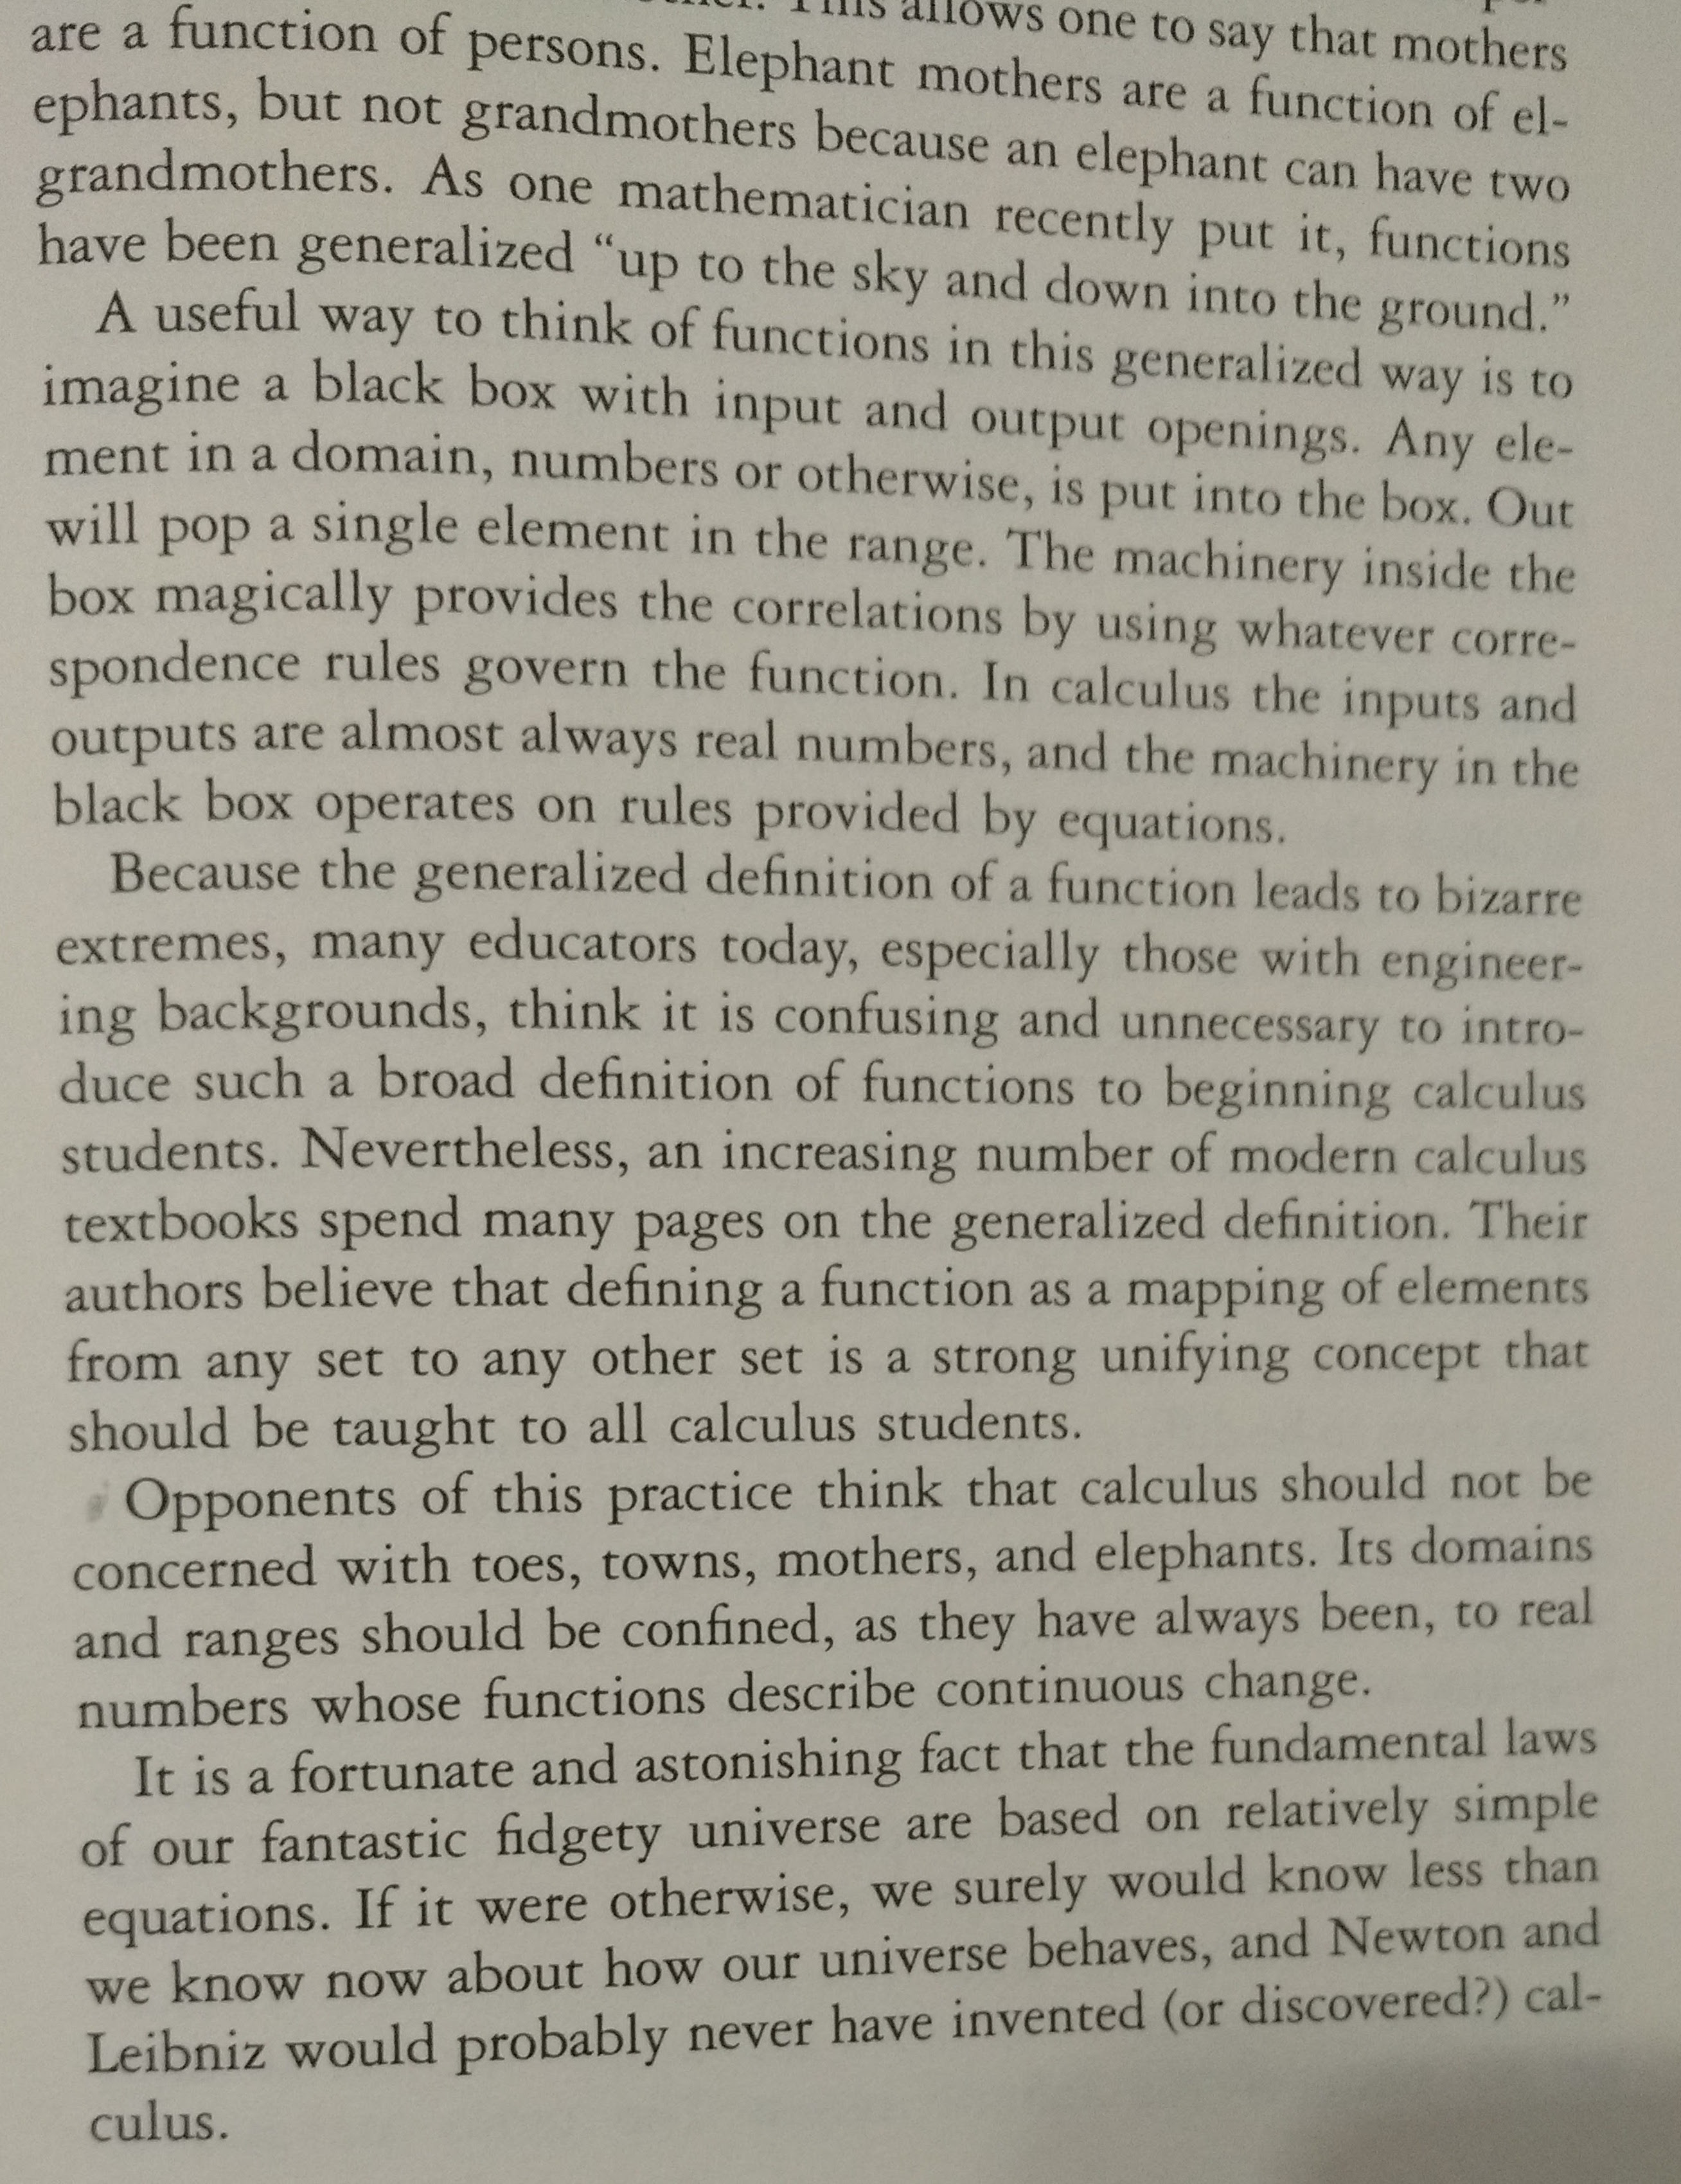
\includegraphics[width=1.0\linewidth]{images/cme01.jpg}
% where an .eps filename suffix will be assumed under latex, 
% and a .pdf suffix will be assumed for pdflatex; or what has been declared
% via \DeclareGraphicsExtensions.
\caption{Teaching maths }
\label{cme01}
\end{figure}

\topic{A sum of all chapters by Thompson}%
{The title is just brilliant and motivating. See \ref{cme01} and \ref{cme03}. We can try the concepts of dx and dy by using numbers extremely small. The next chapters show the formal concept of derivative in a very natural way, as well as the origins of the techniques. Examples including variation of the time. The Chain rule, introduced by Thompson as 'useful dodge'. Geometrical meaning of the differentiation - slopes and curves (it also includes the example of a cusp in the graph, explained in a very good way). Maxima and Minima. Curvatures (positive or negative, or none). Partial fractions and inverse functions, an important manipulation tool. The derivative of an inverse function - "in may respects, calculus is an art, rather than a science". The following chapter shows many examples with growth rates and logarithms. Finally the trigonometric functions. Next, partial differentiation. Integration, as a sum of little triangles or as the reverse of differentiating. Finding areas and volumes. Quadratic mean with integrals. There's a chapter called "Dodges, Pitfalls and Triumphs": Dodges - Rationalization, Factorization and Denominator; Pitfalls - \( 0/0 \); Triumphs - differential equations (brilliant introduction). Finding the length of an arc in a curve using integrals. Hyperbolic and irrational quadratic functions (the exercises here became hard!) That's the end of the book! see \ref{cme04}. There's an appendix with Gardner's notes on recreational problems in mathematics involving calculus [I would always expect something about recreational mathematics coming from Mr. Gardner]. }%

\begin{figure}[!t]
\centering
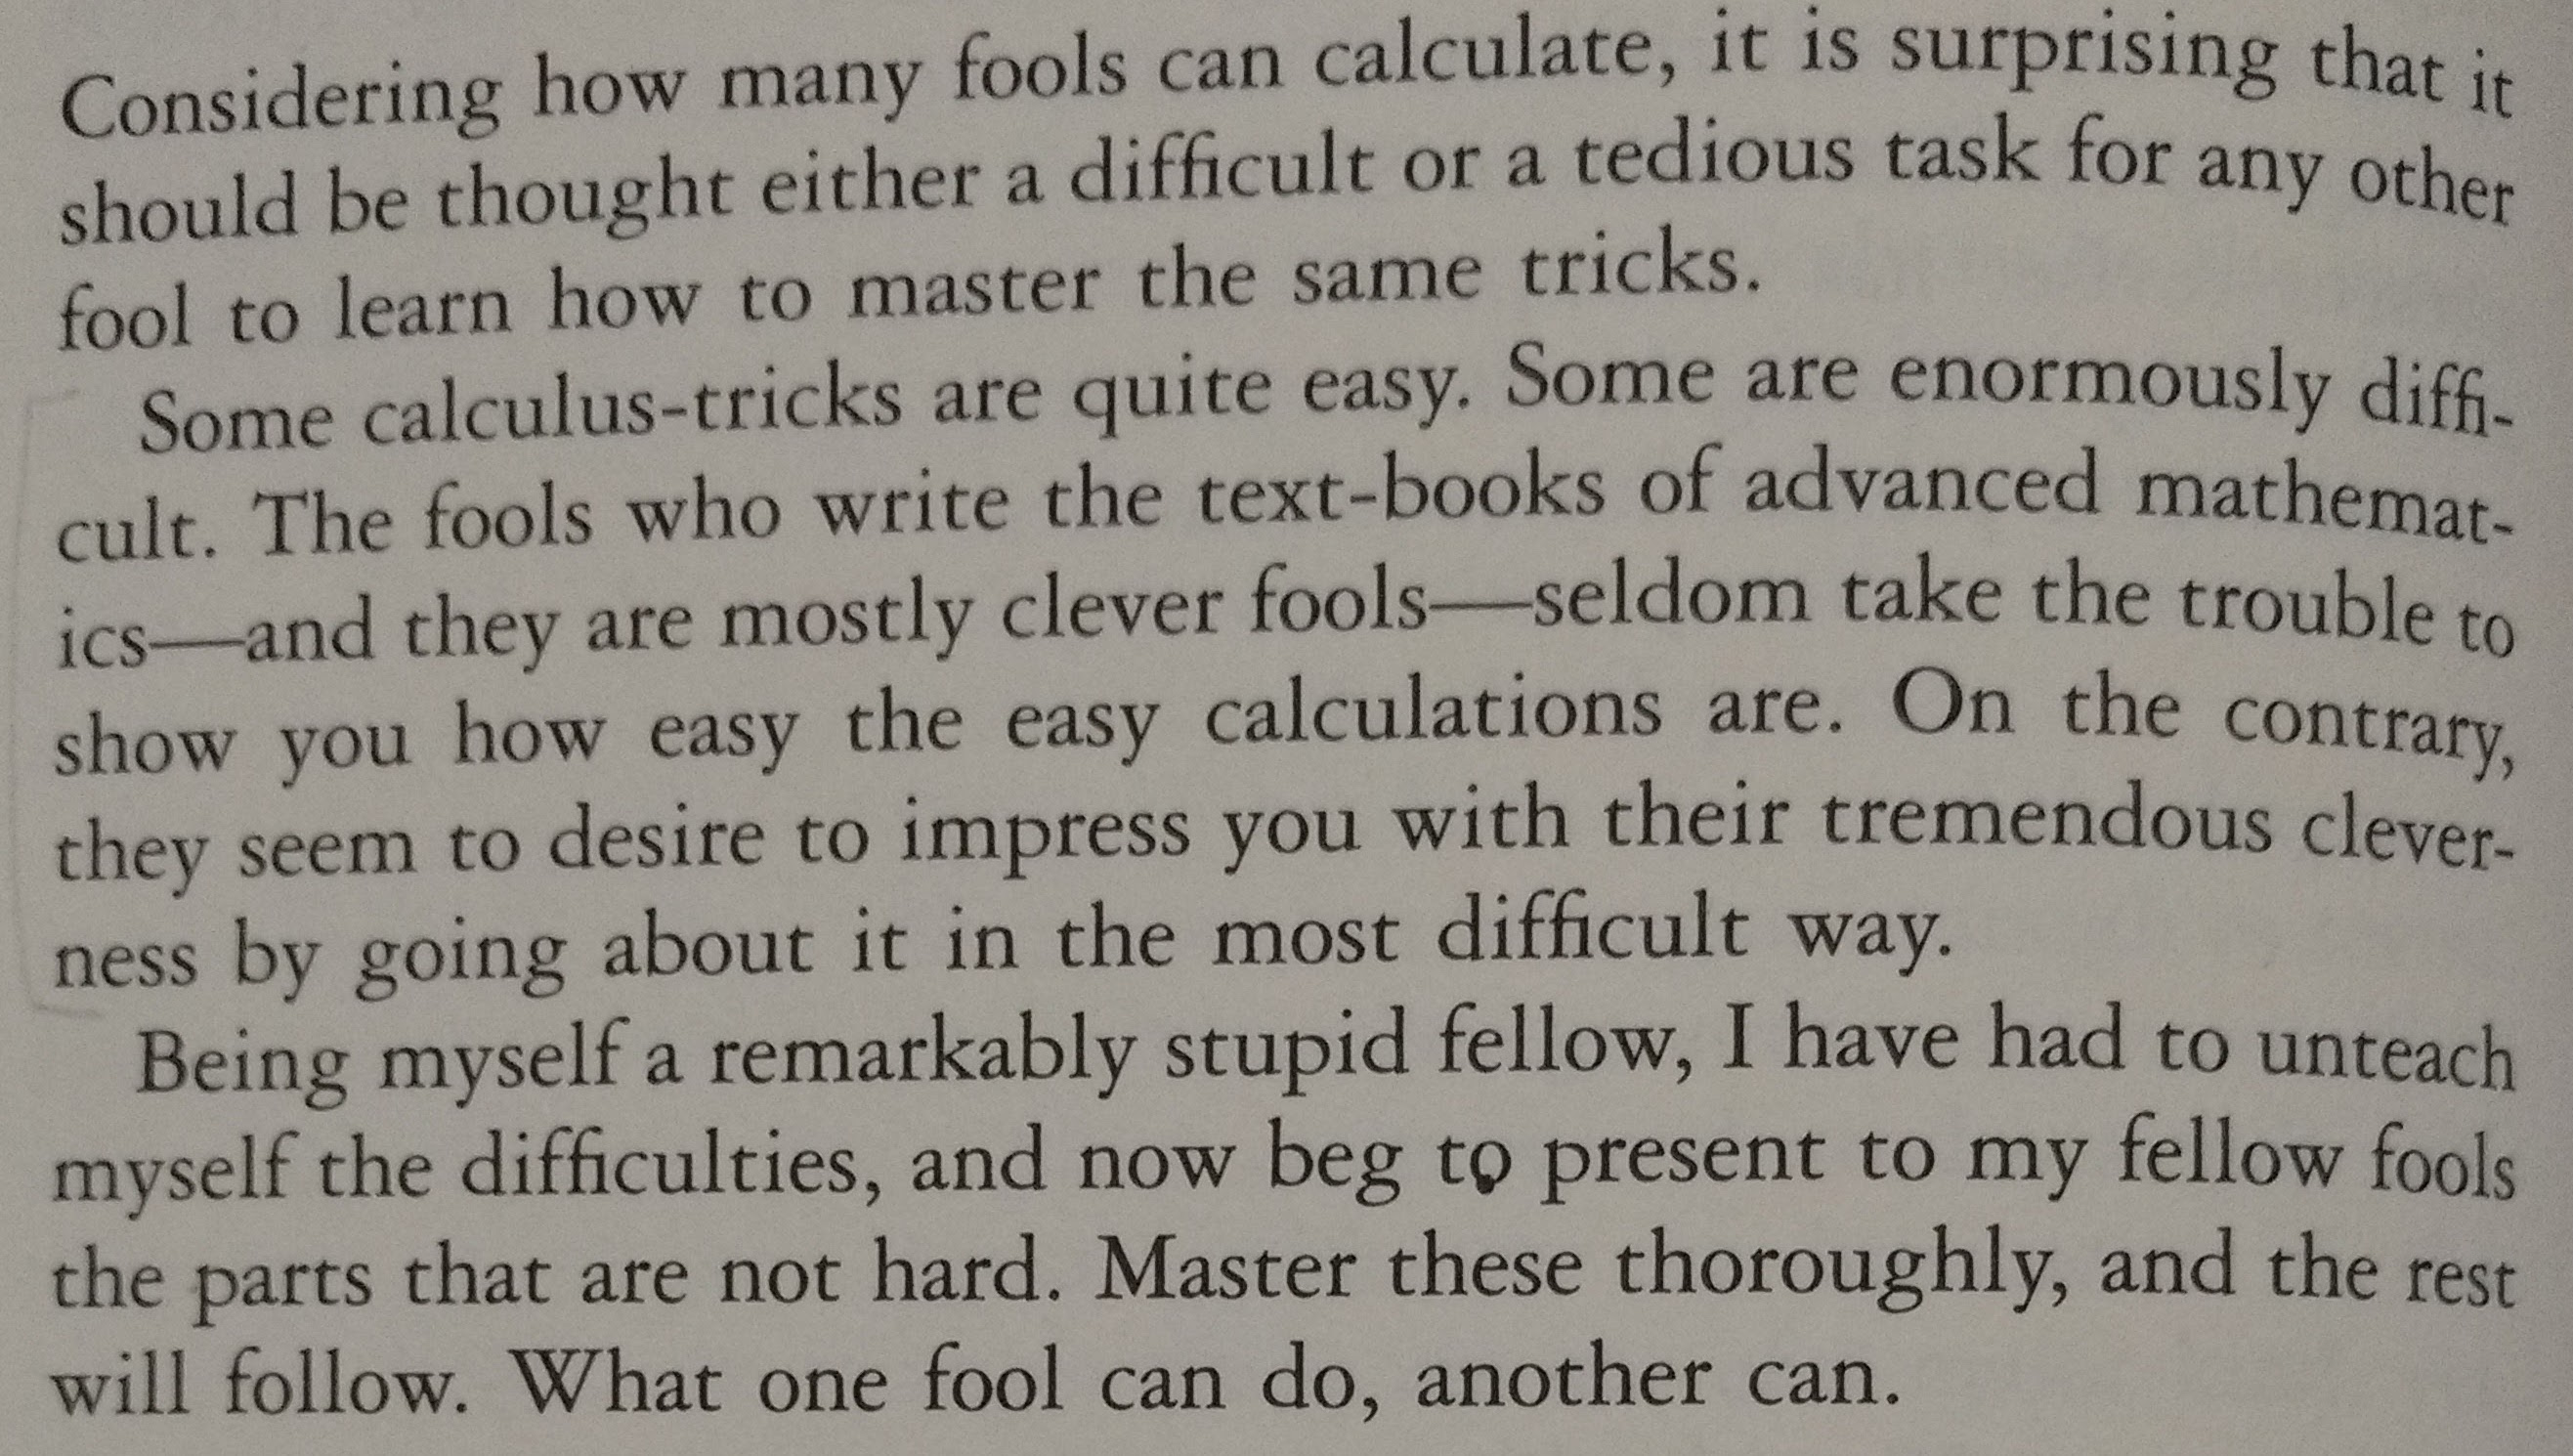
\includegraphics[width=1.0\linewidth]{images/cme02.jpg}
% where an .eps filename suffix will be assumed under latex, 
% and a .pdf suffix will be assumed for pdflatex; or what has been declared
% via \DeclareGraphicsExtensions.
\caption{We can do it }
\label{cme02}
\end{figure}

\begin{figure}[!t]
\centering
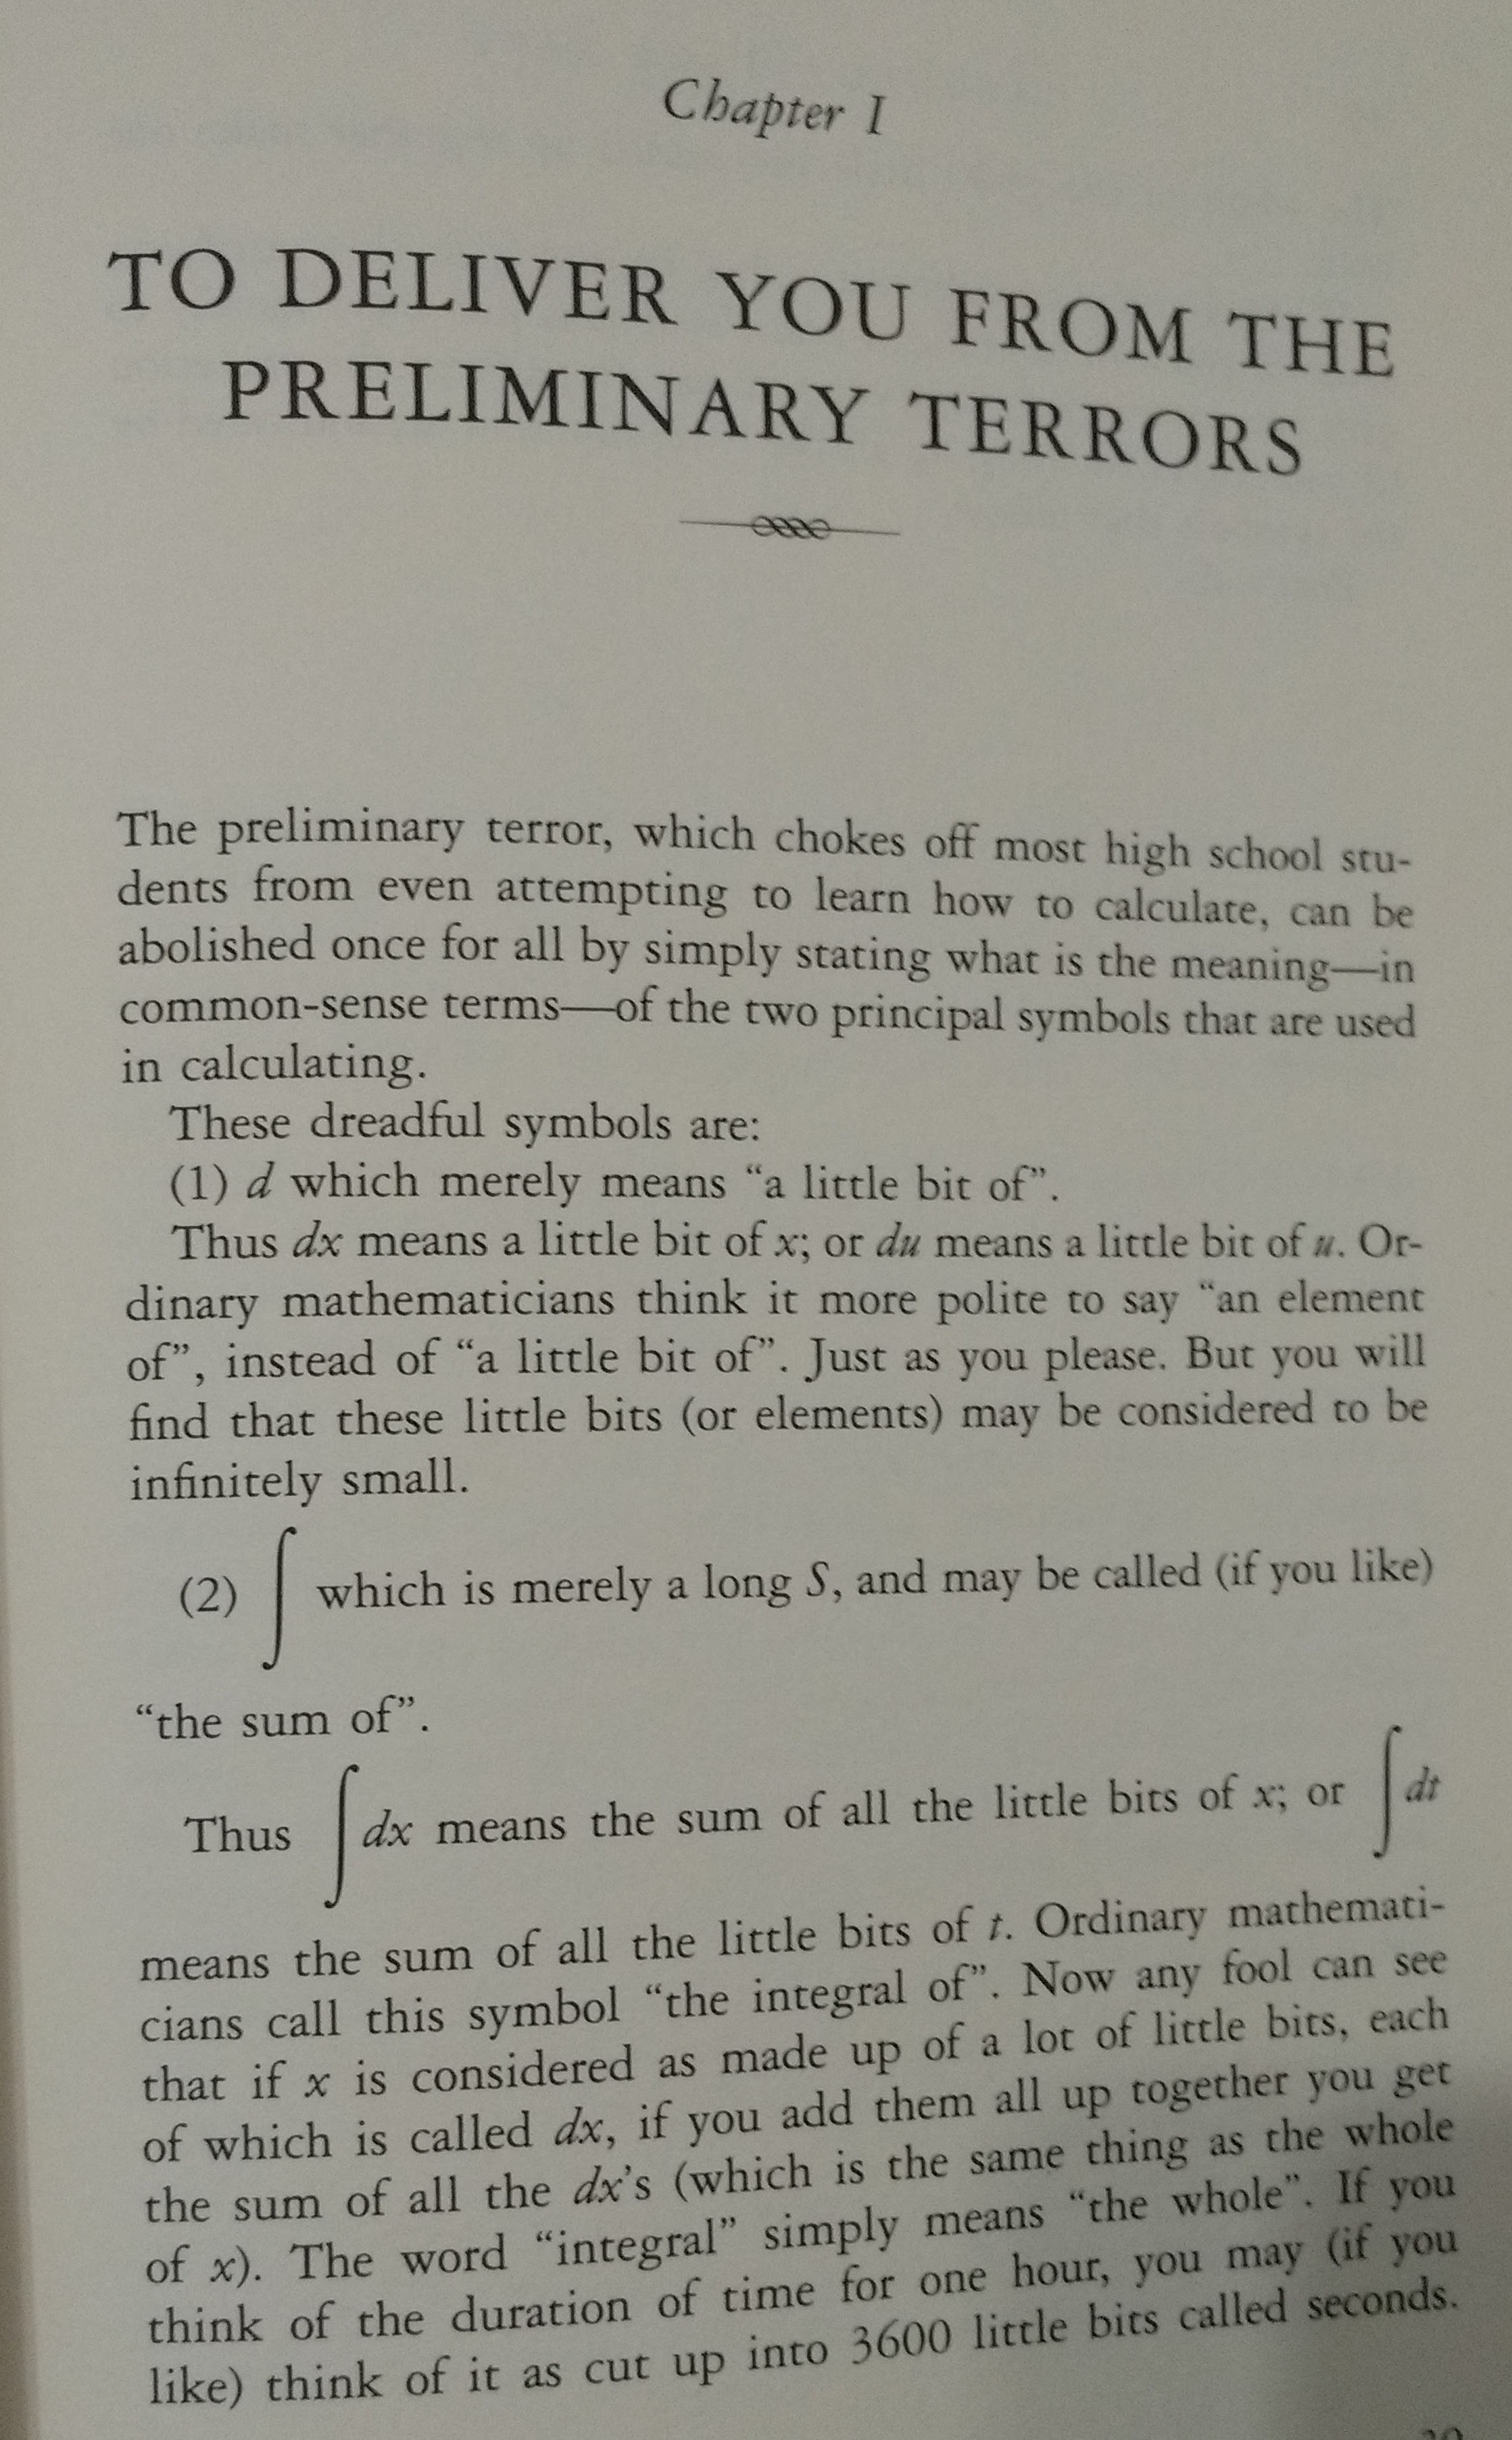
\includegraphics[width=1.0\linewidth]{images/cme03.jpg}
% where an .eps filename suffix will be assumed under latex, 
% and a .pdf suffix will be assumed for pdflatex; or what has been declared
% via \DeclareGraphicsExtensions.
\caption{Short, straight, human-readable definitions }
\label{cme03}
\end{figure}


\summary{I wish I had read this book when I was 15. It is really insightful. Calculus is made easy. :)}



\end{document}